\documentclass[11.5pt]{sig-alternate} % sets document style to sig-alternate
% packages
% typesetting
%\usepackage{dirtytalk} % typset quotations easier (\say{stuff})
\usepackage{hanging} % hanging paragraphs
\usepackage[defaultlines=3,all]{nowidow} % avoid widows
\usepackage[pdfpagelabels=false]{hyperref} % produce hypertext links, includes backref and nameref
\usepackage{xurl} % defines url linebreaks, loads url package
\usepackage{microtype}
%\usepackage[super]{nth} % easily create superscript ordinal numbers with \nth{x}\
\usepackage{enumitem}
% layout
\usepackage{enumitem} % control layout of itemize, enumerate, description
\usepackage{fancyhdr} % control page headers and footers
\usepackage{float} % improved interface for floating objects
%\usepackage{multicol} % intermix single and multiple column pages
% language
\usepackage[utf8]{inputenc} % accept different input encodings
\usepackage[english]{babel} % multilanguage support
% misc
\usepackage{graphicx} % builds upon graphics package, \includegraphics
%\usepackage{lastpage} % reference number of pages
%\usepackage{comment} % exclude portions of text (?)
\usepackage{xcolor} % color extensions
\usepackage[backend=biber, style=apa]{biblatex} % sophisticated bibliographies % necessary for HTML to display author info and date on abstract page
\usepackage{csquotes} % advanced quotations, makes biblatex happy
\usepackage{authblk} % support for footnote style author/affiliation
% tables and figures
\usepackage{tabularray}
%\usepackage{array} % extend array and tabular environments
\usepackage{caption} % customize captions in figures and tables (rotating captions, sideways captions, etc)
%\usepackage{cuted} % allow mixing of \onecolumn and \twocolumn on same page
\usepackage{multirow} % create tabular cells spanning multiple rows
%\usepackage{subfigure} % deprecated, support for manipulation of small figures
%\usepackage{tabularx} % extension of tabular with column designator "x", creates paragraph-like column whose width automatically expands
%\usepackage{wrapfig} % allows figures or tables to have text wrapped around them
%\usepackage{booktabs} % better rules
% dummy text
%\usepackage{blindtext} % blind text dummy text
%\usepackage{kantlipsum} % Kant style dummy text
\usepackage{lipsum} %lorem ipsum dummy text
% other helpful packages may be booktabs, longtable, longtabu, microtype

\pagestyle{fancy} % sets pagestyle to fancy for fancy headers and footers

% header and footer
% modern way to set header image
\renewcommand{\headrulewidth}{0pt} % defines thickness of line under header
\renewcommand{\footrulewidth}{0pt} % defines thickness of line above header
\setlength\headheight{80.0pt} % sets height between top margin and header image, effectively moves page contents down
\addtolength{\textheight}{-80.0pt} % seems to affect the lower height. maybe only works properly if footer numbers enabled?
\fancyhf{}
\fancyhead[CE, CO]{
\includegraphics[width=\textwidth]{headerImage.png}}
% footer
%\fancyfoot[LE,LO]{Article Title Here \\ DOI: }% left footer article title and doi
%\fancyfoot[CE,CO]{{}} % center footer empty
%\fancyfoot[RE,RO]{\thepage} % right footer page numbers
%\pagenumbering{arabic} % arabic (1, 2, 3) numbering in footer

\hypersetup{colorlinks=true,urlcolor=blue} % sets link color to blue
\urlstyle{same} % sets url typeface to same as rest of text

% set caption and figure to italics, label bold, left align captions, does not transfer to HTML
\DeclareCaptionFormat{custom}
{
    \textbf{\textit{\large #1#2}}\textit{\large #3} % #1 is the "Table 1" or "Figure 1" part, #2 is the separator (":"), #3 is the caption
}
\captionsetup{format=custom}
\captionsetup{justification = raggedright, singlelinecheck = false}

%this next bit is confusing, but essentially changes the width of the abstract. Seems to have been copied from this https://tex.stackexchange.com/questions/151583/how-to-adjust-the-width-of-abstract
\let\oldabstract\abstract
\let\oldendabstract\endabstract
\makeatletter %changes @ catcode to enable modification (in parsep)
\renewenvironment{abstract} %alters the abstract environment
{\renewenvironment{quotation}%
               {\list{}{\addtolength{\leftmargin}{1em} % change this value to add or remove length to the the default ?
                        \listparindent 1.5em%
                        \itemindent    \listparindent%
                        \rightmargin   \leftmargin%
                        \parsep        \z@ \@plus\p@}%
                \item\relax}%
               {\endlist}%
\oldabstract}
{\oldendabstract}
\makeatother %changes @ catcode to disable modification

\begin{document}

\title{Students’ with Blindness and Visual Impairments Level of Engagement in Science and Engineering Practices}

\author[1]{\large \color{blue}Tiffany A. Wild}
\author[1]{\large \color{blue}Danene K. Fast}
\author[2]{\large \color{blue}Karen Koehler}
\author[3]{\large \color{blue}Natalie Shaheen}
\author[1]{\large \color{blue}Julia Averill}
\author[4]{\large \color{blue}Kathleen Farrand}

\affil[1]{The Ohio State University}
\affil[2]{Shawnee State University}
\affil[3]{Illinois State University}
\affil[4]{Arizona State University}


\toappear{}
%% ABSTRACT
\maketitle
\begin{@twocolumnfalse} 
\begin{abstract}
\item 
\textit {There is a lack of research on science-process skills and abilities of students with blindness and visual impairments to apply those skills (Jones, Forrester, Robertson, Gardner, \& Taylor, 2012). This study aims to provide additional information on how students with blindness and visual impairment are engaged in science and engineering practices in order for teachers to gain a better understanding of how students with visual impairments can learn engineering practices. The Student Inquiry Review (Hilson \& Wild, 2015) that examines the scientific and engineering practices as defined in the Framework for K-12 Science Education: Practices, Crosscutting Concepts and Core Ideas (National Academy of Sciences, 2012) was used for this study. Specifically, researchers examined the eight defined science and engineering behaviors of students with visual impairments as they were engaged in a science curriculum specifically designed for them.}
\\ \\
Keywords: Visual Impairment, Science, Engineering
\end{abstract}
\end{@twocolumnfalse}

%% AUTHOR INFORMATION

\textbf{*Corresponding Author, Tiffany A. Wild }\\
\href{mailto: wild.13@osu.edu }{(wild.13@osu.edu)} \\
\textit{Submitted January 23, 2019 }\\
\textit{Accepted December 3, 2019} \\
\textit{Published online January 14, 2020} \\
\textit{DOI:10.14448/jsesd.12.0016 
}
\pagebreak
\clearpage

\begin{large}
\section*{INTRODUCTION}

The field of engineering incorporates both science and mathematics. Students need to be engaged in science while using mathematical skills to support inquiry, design, and communication of results with others. Science and mathematics are often taught in the general education curriculum using visual methods, which make it difficult for students with visual impairments to access. According to Gottfied et al. (2016), students with disabilities, including those with sensory impairments, are taking less advanced coursework in mathematics and science than those in the general population. This research indicates that students with disabilities do not develop the foundational knowledge in science and mathematics that would allow for success in advanced courses. Without this basic knowledge, engineering can be difficult for students with visual impairments.  

Engineering Education is needed now more than ever. According to Draxler (2013) “Our society depends upon engineers to design every aspect of our lives – where we live, what we drive, how we communicate and even what we eat – but America’s primary and secondary education systems aren’t producing enough critical thinkers to keep up with the demand” (para. 4). The Next Generation Science Standards (Achieve, 2013), integrate engineering practices into the K-12 science classroom. Every grade level and subject area has reference to science and engineering practices that are appropriate to the content suggested. The rationale for including engineering practices into the standards is to not only pique interest in motivation but also to better understand that science and research is a creative process that impacts the world (NRC, 2012). The emphasis is on the process, not the memorizing of scientific facts. Without doing so, according to the NRC “…ignores the many important applications of science in the world misrepresents science and marginalizes the importance of engineering” (p. 43).  

\subsection*{Rationale}

There is a lack of research on science-process skills and abilities of students with blindness and visual impairments to apply those skills (Jones, et al., 2012). Numerous studies exist to show engagement in science. The few research studies that have been conducted concerned adaptations made to specific curricula and science equipment (Erwin, et al., 2001; Wild \& Trundle, 2010a; Wild \& Trundle, 2010b). These studies do not reflect the current standards and trends in science education (Gough, 1978; Linn \& Their, 1974; Long, 1975; Struve, et al., 1975; Waskoskie, 1980).  Instructional techniques have been reported for teaching the concepts for scale, environmental science, biodiversity, seasonal change, space, sound, and geoscience to students with visual impairments (Jones, et al., 2008; Wild \& trundle, 2010a; 2010b; Rule, 2011; Wild, et al., 2013; Wild, et al., 2013; Hilson et al., 2016; Koehler et al., 2018). There is little replication in the work and therefore one cannot assume any one technique for teaching specific content is appropriate. In the review of literature for this paper, only one study showed engagement in science and engineering practices (Hilson \& Wild, 2015). Jones et al. (2012), suggest that more research is needed to understand how students with visual impairments learn science. “We cannot afford for any child not to be knowledgeable about science, regardless of whether they become scientists or not” (Jones, et al., 2012, p. 355). This study aims to provide additional information on how students with blindness and visual impairment are engaged in science and engineering practices in order for teachers to gain a better understanding of how students with visual impairments can learn engineering practices. 

\section*{CURRICULUM}

The curriculum for the engineering program was grounded in the Engineering Design Process Portfolio Scoring Rubric (EDPPSR) (Goldberg, 2014), which was developed as part of another project funded by the National Science Foundation. Each element of the EDPPSR is aligned with a stage of the engineering design process (e.g., identifying a problem, developing in an initial solution, building a prototype, analyzing data, and re-designing). Each lesson in the program curriculum aligned to at least one element of the EDPPSR. For example, early lessons  in the program, which introduced students to the problem and provided them with data they could use to better understand the problem, aligned with Element A from the EDPPSR—presentation and justification of the problem (Goldberg, 2014). Lessons presented later in the curriculum where students brainstormed a handful of possible solutions to the problem (e.g., watercraft designs) and later identified the best design addressed Element D from the EDPPSR—design concept generation, analysis, and selection (Goldberg, 2014).

The researchers did not help in the design or implementation of the curriculum. A collaborative team of blind scientists, experts in the field of visual impairment, and science education designed the curriculum from the ground up to be nonvisually accessible to ensure that students with blindness and visual impairments could participate fully in all of the learning. Four specific examples of the curriculum’s built-in accessibility follow. First, students had access to all instructional materials in Braille, large print, and accessible electronic formats. Second, for each activity, teachers provided hands-on instruction in how to perform essential skills and techniques (i.e., how to fasten PVC or how to collect turbidity data); during this instruction, students were encouraged to tactually observe teachers’ demonstrations—putting their hands over the teachers’ hands. Third, students used nonvisually accessible laboratory equipment (e.g., SciVoice Talking LabQuest©, click rule) to collect data. Fourth, students had ready access to accessible communication tools (e.g., Braille writers, Braille embossers, bold line pens and paper, computers with screen access software), which are essential for students with blindness and visual impairment to demonstrate their understanding.

The curriculum focused on three tasks that were related through a fictitious real world problem students were asked to solve. The three major tasks were: designing and constructing a watercraft out of commonly available materials (e.g., PVC pipe, tarps, duct tape), designing and constructing a water filtration system out of commonly available materials, and drafting graphical representations of their design solutions using orthographic and isometric projections. The overall goals of the curriculum were consistent across iterations of the program, but the instructional design evolved over the course of the grant in response to feedback from external evaluators and students as well as the instructors’ observations of the students’ engagement with the various learning activities. The greatest shift in the curriculum occurred between session one and two with only small tweaks to the curriculum between session two and three.  

The changes to the instructional design from session one to session two centered around increasing student inquiry, specifically increasing students’ opportunity to engage with the iterative engineering design process. For example, in session one all student teams worked off of the same watercraft design, building from existing plans rather than generating their own designs. In session two and three, students were given design requirements and constraints and tasked with developing their own watercraft design. To provide students with the necessary prior knowledge to be successful in the watercraft design activity, students participated in a modeling and inquiry activity where they developed an understanding of Archimedes’ principle and how it relates to various hull shapes (e.g., V-hull, displacement hull, and flat-bottomed hull). Students then used their understanding to develop possible hull designs at a smaller scale using dowels and 3-D printed fittings. These designs, which mimicked the shape of the PVC pipe fittings they would later use in their full-size watercraft, were used to construct their mini hulls and then to test their designs in a hydrostatic bin (e.g., a large plastic bin with a spout at the bottom). In this activity, students had the opportunity to iterate their designs at a small scale based on the data they collected and analyzed when they tested their hull in the hydrostatic bin. The understanding that students developed from the mini hull design activity was later used to engineer their full-scale watercraft prototype. 

Another change to the instructional design between sessions one and two that facilitated greater engagement with the engineering design process was access to a test pool throughout the week. Once students had constructed their full-scale prototype, they were able to test their prototype in the pool and determine how their design could be improved. In the first session, a test pool was not available throughout the week, which limited students’ opportunity to iteratively design their full-scale watercraft. A similar prototype testing sequence was used in the development of the water filtration systems. Students developed prototype filters, ran contaminated water through the filters, and then collected data related to the potability (e.g., coliform bacteria, nitrite, pH, dissolved solids) of the filtered water. Students used the understanding they developed through their prototype testing to design their final water filtration system. 

\begin{figure}[h]
    \centering
    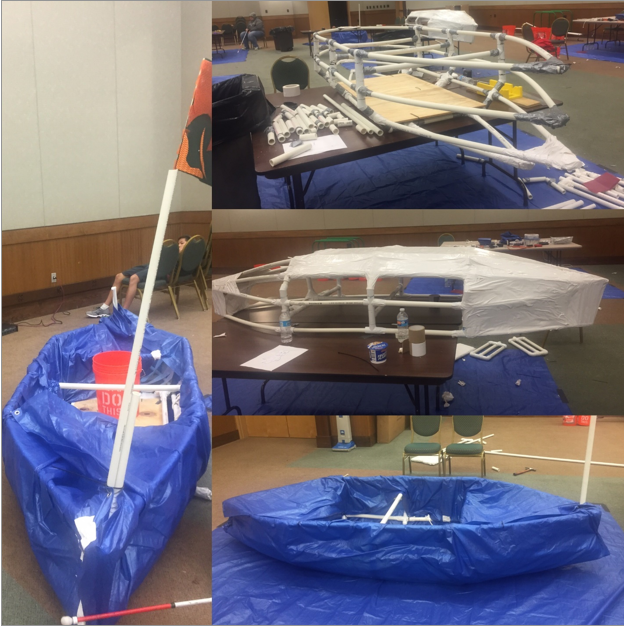
\includegraphics[width=1\linewidth]{fig1.png}
    \caption{Boat Design Collage from Programming}
\end{figure}

\begin{figure}[!h]
    \centering
    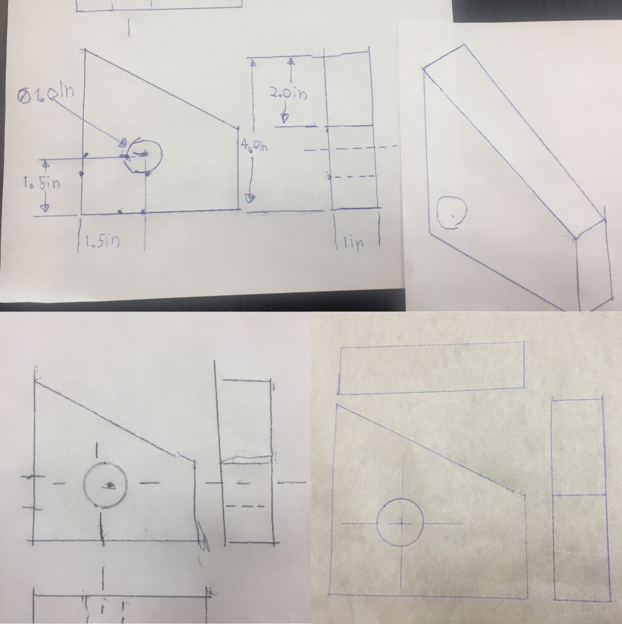
\includegraphics[width=1\linewidth]{fig2.png}
    \caption{Student Sketch of Wooden Block Practicing Orthographic Projection}
\end{figure}

\begin{figure}[!h]
    \centering
    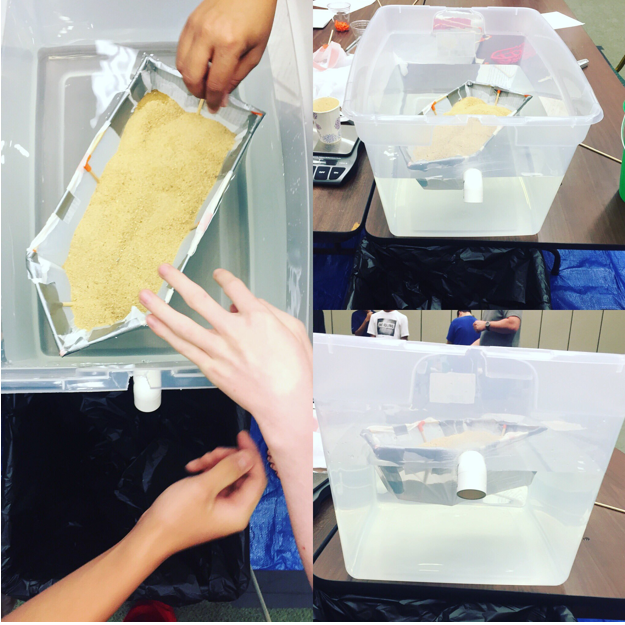
\includegraphics[width=1\linewidth]{fig3.png}
    \caption{Hydrostatic Bin Images}
\end{figure}

\newpage

\section*{METHODOLOGY}

The Ohio State University Institutional Review Board approved all methods used to collect data in this study.  

\subsection*{Participants}

Student participants self-selected to attend the summer program described above. All students in the program were provided the opportunity to participate in the research study through recruitment materials mailed after enrollment had been confirmed, but prior to the beginning of the program.  

The program leaders verified that all students that were enrolled in the program had blindness or a visual impairment. Acuity levels of vision or reading media used was not part of the data collection process by the researchers as well as any additional disabilities or medical information. This information was not made available to the researchers by the program leaders as part of terms of agreement for the research.      

All participants in this study provided written consent from either their parents, or self-consent if over 18. Twenty-seven students with visual impairments participated in this study over three sessions. Nine students were members of session one, 13 in session two and 5 in the last session. All participants self-selected to attend this summer program. Participants were high school aged and ranged from 9th to 12th grade. Ages of the students ranged from 14-19 years.   

See table 1 for more demographic information.

\begin{table*}[t]
\caption{Student Demographics}
\begin{tabular}{p{2in}p{2.5in}p{2.5in}p{2.5in}}
Demographic & Summer Session 2015 Participants & Summer Session 2016A Participants & Summer Session 2016B Participants \\ \hline
Age & & & \\
14 & 0 & 1 & 0 \\
15 & 0 & 1 & 0 \\
16 & 4 & 4 & 1 \\
17 & 4 & 3 & 4 \\
18 & 0 & 4 & 0 \\
19 & 1 & 0 & 0 \\
Gender & & & \\
Female & 4 & 3 & 4 \\
Male & 5 & 10 & 1 \\
Ethnicity & & & \\
African American & 0 & 1 & 0 \\
Asian & 4 & 2 & 1 \\
Caucasian & 3 & 7 & 4 \\
Chinese & 2 & 0 & 0 \\
Hispanic & 0 & 2 & 0 \\
Other & 0 & 1 & 0 \\
Grade & & & \\
9 & 0 & 2 & 0 \\
10 & 1 & 3 & 3 \\
11 & 5 & 4 & 2 \\
12 & 3 & 4 & 0 \\
\end{tabular}
\end{table*}

\subsection*{Instrument}

The Student Inquiry Review (Hilson \& Wild, 2015) was used in this research. The curriculum from this program leant itself nicely to observing the engineering behaviors of students. The Student Inquiry Review (SIR) instrument requires researchers to examine the scientific and engineering practices as defined in the Framework for K-12 Science Education: Practices, Crosscutting Concepts and Core Ideas (National Academy of Sciences, 2012). Specifically, researchers examine the behavior of students engaged in science and engineering practices in 5-minute intervals for a total of 30 minutes. Observations were made randomly among the students working in small groups during the curriculum delivery. Specifically, researchers examined 8 behaviors  
\newpage
\begin{enumerate}[nosep]
    \item Asking questions and defining problems
    \item Developing and using models
    \item Planning and carrying out investigations
    \item Analyzing and interpreting data
    \item Using mathematics and computational thinking
    \item Constructing explanations and designing solutions
    \item Engaging in written and oral argument from evidence
    \item Obtaining, evaluating, and communicating information (National Academy of Science, 2012; Hilson \& Wild, 2015)
\end{enumerate}

Included in the instrument, was additional space for notes to document the activities. Any behaviors of the student observed during the observational time was explained and documented on page 2 of the instrument. 

The 8 behaviors are based on the science and engineering practices developed in \textit{A Framework for K-12 Science Education: Practices, Crosscutting Concepts, and Core Ideas} (NRC, 2012). The behaviors define how inquiry should be conducted in k-12 settings and emphasize practicing like a scientist rather than reading about science or watching others employ science practices.  

For the first behavior, asking questions and designing problems, the focus is on the problem that needs to be solved. What questions need to be asked in order to solve a given problem in society?

The second behavior, developing and using models, requires students to be engaged in using models and simulators to test or analyze possible solutions to the existing problems defined in the first behavior.

The third behavior, planning and carrying out investigations, allows engineers to gain data. Engineers must define the variables; decide how the investigation will be carried out, how data will be collected, and how data will be analyzed. This is methodology planning that naturally occurs in an investigation.  Once the plan is made, engineers carry it out. Data and observations are collected.  

After the testing, comes the analyzing and interpreting of data. In this phase, data sets are compared and different solutions to the problem are compared to determine the best solution to the problem defined at first. This requires many tools such as graphs, statistics, and visualizations.

After analysis comes the use of mathematics and computational thinking to calculate data within the problem. Many times this is visible when engineers use mathematics and computations to establish relationships that will allow for a prediction of the answer to the problem and predict possible outcomes.  

Constructing explanations and designing solutions is the point in the process where proposed solutions result. There is usually no best solution, but many for which engineers must choose the best possible solution given the criteria and outcomes. “Each proposed solution results from a process of balancing competing criteria of desired functions, technological feasibility, cost, safety, esthetics and compliance with legal requirements” (NRC, 2012, p. 52).

Once a solution is found, one must engage in argumentation based upon the evidence. Many times engineers work with peers to solve problems. At this point in the problem solving process engineers compare their work with others and prepare to make arguments of their findings based upon data. The engineers engage in critical examination of each other’s’ work and revise any ideas in order to get the possible solution to the original problem.  

The last step is to obtain, evaluate and communicate the information to others. Engineers need to be able to share their work and ideas with others using oral and written communication which can also include graphs and models. Engineers need to be able to discuss ideas with their peers and obtain information so that the knowledge can be applied to new problems. Thus begins the cycle again. 

\subsection*{Data Analysis}

Data analysis focused on frequency and application of each of the eight behaviors documented and observed using the SIR instrument. Examples of each of the eight behaviors were noted to provide further documentation of the category chosen for the time interval that focused on the curriculum and/or activity of the students.  

\section*{FINDINGS}

For the first behavior, asking questions and designing problems, the students’ behaviors observed included asking instructors for specific information regarding the problems given. For example, one student observed was asking the instructors about the basic principles of buoyancy displacement so that he could begin work on his boat design. Another student was observed asking questions of a partner in order to determine constraints in the boat design.

The second behavior, developing and using models, was observed as students began to plan their boat model design. One student was observed drawing plans while another was observed building prototypes of boats and testing for buoyancy and displacement of water. Yet another student was observed drawing a design for a boat paddle and laying out connectors for the paddle design with PVC pipe, fitting the pipe to his boat.

The third behavior was observed many times throughout the curriculum. This was seen as students tested water for various components, such as pH and dissolved oxygen, and then filtering and re-filtering the water to remove impurities. Another example was when the students’ tested their finalized boat models.

After the testing, students were observed analyzing and interpreting their data. One student was observed using the Vernier© probes and talking LabQuest© to measure dissolved solids, dissolved oxygen and ph. This student analyzed the data collected to figure out if the design of the filtration unit worked successfully.

After analysis comes the use of mathematics and computational thinking to calculate data within the problem. For example, one observation noted in this category was of a student determining that measurements he made of the group’s filtered water were in the acceptable range for drinking. Another student used measurement data to determine the ratio of his model paddles and boats to an actual paddle and boat.  

Constructing explanations and designing solutions was frequently observed as students worked to explain to their small groups the design for their boats and paddles. As a result, students were also observed discussing adjustments that needed to be made to their original designs. Another example was when students discussed ways they could change their filtration system so that it would remove bacteria detected in the water. Similarly, another student group engaged in adding gravel, charcoal, and sand in order to improve on the design of their water filtration system.

Once the students had their designs and data, they needed to engage in written and oral argument. Students were observed documenting test results in a lab report, arguing and answering questions of the instructors in order to defend their design, and small group discussions of the best filter system.

\begin{table*}[t]
\caption{Tally of Student Behavior}
\begin{tabular}{p{3in}p{2in}p{2in}p{2in}}
Student Behavior & Session \#1 & Session \#2 & Session \#3 \\
 & N=9 & N=13 & N=5 \\ \hline
Asking questions and defining problems & 35 & 33 & 9 \\
Developing and using models & 24 & 74 & 16 \\
Planning and carrying out investigations & 18 & 35 & 26 \\
Analyzing and interpreting data & 5 & 11 & 11 \\
Using mathematical and computational thinking & 1 & 54 & 20 \\
Constructing explanations and designing solutions & 8 & 49 & 34 \\
Engaging in written and oral argument with evidence & 1 & 17 & 7 \\
Obtaining, evaluating, and communicating information & 20 & 73 & 64 \\
\end{tabular}
\end{table*}

The last behavior observed was of obtaining, evaluating, and communicating information. This behavior was observed as students discussed with other groups their results and communicated their results to specialists or the instructors. This behavior was an engagement between the students and experts about information learned throughout their investigations. The tally of student engineering behaviors can be found on Table 2.

During the first summer session, most of the time the students were observed asking questions and defining problems. Teams were engaged with asking questions about tasks that were part of the curriculum such as the design of the water filtration system, posing questions to experts that could inform the team of model development, and asking guidance questions about use of materials as part of their investigations. The teams also spent a large amount of time developing and using models. Teams were engaged in designing water filtration systems and using the models in various tests and creating their boat models. The least observed behavior was that of engaging in written and oral argument from evidence. This was only captured once when a student was engaged in giving a group presentation on the work that was completed through the week. Another area that was not well represented was that of using mathematical and computational thinking. This behavior was observed when a student was trying to determine the length of a paddle handle and the surface area of the paddle. The student used a ruler to measure lengths.   

During session two, students were most frequently seen developing and using models. Teams were observed using 3-D models to help in constructing their own models. Development of models were most frequently linked with the next highest observed category of obtaining, evaluating and communicating information. This observation reflects time spent learning from instructors, working as a team to discuss ways to problem solve unexpected data results, and discussing plans for each design challenge presented. This group also spent much time on using mathematical and computational thinking. Much of this was seen in group work of making measurements as each group designed their boat and interpreting scale from the model to actual building of the boat and paddles. The least frequently observable behavior was that of engaging in written and oral argument from evidence. This was observed at the end of the week when students were observed preparing reports of the work they had completed during the week.  

During the final summer session, students were most frequently engaged in obtaining, evaluating, and communicating information. Students were working as a team to discuss their projects. Students were also working to get more information from instructors that would improve their projects. Frequent documentation revealed students evaluating the angles of the boats, or immersed in discussion regarding changes in design. Students also spent time discussing how they would communicate the information learned in the curriculum with others. The least frequently observed behavior was engaging in written and oral argument with evidence.  

\section*{LIMITATIONS}

This study was conducted with a convenience sample of students that volunteered and chose to attend this program. Since participants self-selected into the program, the results may be skewed to academic students who had an interest in science and engineering and thus may have influenced the findings. No random sampling or treatment were applied. The results were based solely on observation. The results cannot be generalizable to the larger population of students with visual impairments.  

The instrument allowed an observer to focus on one student for 30 minutes. Depending on when that observation occurred, some students may have not been fully engaged in any of the activities of the team and therefore no behaviors were observed or working independently on something unrelated to the process skills. For example, for 30 minutes one student was observed creating a team flag.  Ultimately, this can skew the data to infer students were not fully engaged in the science and engineering practices, which were the focus of the program. However, it is important to note that all behaviors were observed during each program session.

The curriculum changed slightly between sessions. Therefore, behaviors between sessions changed to reflect the change in curriculums. Sessions two and three had students more engaged in the science and engineering practices. This engagement can be seen as a direct change in the curriculum implementation.  

The authors acknowledge the gap between the data collection and preparation of manuscript for publication. Extenuating circumstances in the research team caused delays in preparation. However, the information contained within the manuscript, and a lack of similar work in the field, warranted the team to continue to seek publications of findings.  

\section*{CONCLUSIONS AND IMPLICATIONS}

Similar to the previous work by Hilson and Wild (2015), students were observed carrying out all eight of the engineering and science practices. The frequencies of which students with visual impairments were engaged in these activities differed from previous research (Hilson \& Wild, 2015) of students with visual impairments engagement in engineering and science practices. This research provides a further example of the abilities of students with blindness and visual impairments when given the opportunity to engage in science and engineering with differing lessons and objectives than those described in previous research by Hilson and Wild (2015). While there were also differences in categories of behaviors observed between camp sessions examples of each of the behaviors were observed.  

The findings suggest that students with blindness and visual impairments, when given the opportunity, can fully participate in science and engineering processes when given the proper tools. Students need to be encouraged by their teachers, mentors, or support personnel to engage in written and oral arguments from their evidence more frequently. This could come in the form of presentations at the end of the project that would display their work for the public or through written articles that could be featured in newsletters and other publication opportunities. This in turn could easily promote self-determination and additional skills that would translate into their adult lives. Above all else, teachers need to be sure to give students with visual impairments the opportunity to engage in real-life scientific work, as these students have the ability to do so as evidenced through this research.

Acknowledgement: This research was made possible through funding provided by the National Science Foundation under grant no. 1322855. Sub-award for research from the National Federation of the Blind.  

\end{large}
\include{} 
\section*{REFERENCES}\par 

\leftskip 0.25in
\parindent -0.25in 
Achieve (2013).  Next generation science standards: For states, by states.  National Academies Press: 
Washington, DC.

Draxler, B. (December 2013).  Teaching kids to think like engineers: Engineering instruction should build on young students’ natural problem-solving skills to prepare a future generation of critical thinkers. \textit{Discover Magazine, 34}(10), 56-59.  Available at: \url{https://www.discovermagazine.com/the-sciences/teaching-kids-to-think-like-engineers}

Erwin, E., Perkins, T., Ayala, J., Fine, M., Rubin, E. (2001).  You don’t have to be sighted to be a scientist, do you? Issues and outcomes in science and education. \textit{Journal of Visual Impairment \& Blindness, 95}(6), 338-352.

Goldberg, G. L. (2014). Revising an Engineering Design Rubric: A Case Study Illustrating Principles and Practices to Ensure Technical Quality of Rubrics. \textit{Practical Assessment, Research \& Evaluation, 9}(8), 1-12.

Gottfied, M., Bozick, R., Rose, E., \& Moore, R.  (2016).  Does career and technical education strengthen the STEM pipeline?  Comparing students with and without disabilities.  \textit{Journal of Disability Policy Studies, 26}(4), 232-244.

Gough, E. (1978). \textit{The science-related problem solving processes of visual impaired adolescents}. Unpublished doctoral dissertation, Indiana University.  

Hilson, M. \& Wild, T. (2015).  Science inquiry and students with visual impairments.  \textit{Visual Impairment and Deafblind Education Quarterly, 60}(3), 28-55.  Retrieved from: \url{http://dvi.uberflip.com/i/548082-vidbe-quarterly-volume-60-3}. 

Hilson, M., Hobson, S., \& Wild, T.  (2016).  Conceptual understandings of students with visual impairments about biodiversity across ecosystems.  Journal of Blindness Innovation and Research, 6(2).  Retrieved from: \url{https://nfb.org/images/nfb/publications/jbir/jbir16/jbir0602tc.html}

Jones, M.G., Forrester, J., Robertson, L, Gardner, G., \& Taylor, A. (2012).  Accuracy of estimations of measurements by students with visual impairments.  \textit{Journal of Visual Impairment and Blindness, 106}(6), 351-354. 

Koehler, K.; Wild, T.; and Tikkun, S. (2018) "Implications of 3-D Printing for Teaching Geoscience Concepts to Students with Visual Impairments," \textit{Journal of Science Education for Students with Disabilities, 21}(1), 49-81. Available at: \url{https://scholarworks.rit.edu/jsesd/vol21/iss1/6}

Linn, M. \& Their, H.  (1975).  Adapting science material for the blind (ASMB); Expectation for student outcomes. \textit{Science Education, 59}(2), 237-246. 

Long, N.  (1973).  \textit{Science curriculum improvement study (SCIS): its effect on concept development and manipulative skills in visually handicapped children}.  Unpublished doctoral dissertation.  University of California: Berkeley.   

National research Council (2012).  A Framework for K-12 science education: Practices, Crosscutting Concepts and Core Ideas.  National Academies Press: Washington, DC.

Struve, N., Their, H., Hadary, D., \& Linn, M.  (1975).  The effect of an experiential science curriculum for the visually impaired on course objectives and manipulative skills.  \textit{Education of the Visually Handicapped, 7}(1), 9-14.

Waskoskie, W.  (1980).  \textit{Teaching biology concepts to blind college-level students through audio-tutorial-self-instruct laboratory experiences}.  Unpublished doctoral dissertation.  University of Pittsburgh.  

Wild, T., Hilson, M., Hobson, S.  (March-April, 2013).  Conceptual understandings of sound by students’ with visual impairments.  \textit{Journal of Visual Impairment and Blindness, 107(2)}, 107-116.

Wild, T., Hilson, M., \& Farrand, K. (2014). Preparing for an inquiry-based summer camp experience for students with visual impairments: What do the campers think? \textit{Journal of Blindness Innovation and Research, 4}(2). Retrieved from \url{https://nfb.org/images/nfb/publications/jbir/jbir14/jbir040201.html}.

Wild, T. \& Trundle, K. (2010a).  Talking turkey: Teaching about North America’s greatest observation story with children with visual impairments, \textit{Journal of Visual Impairments \& Blindness, 104}(4), 198-201.

Wild, T. \& Trundle, K.  (2010b).  Conceptual understandings of seasonal change by middle school students with visual impairments, \textit{Journal of Visual Impairment \& Blindness, 104}(2), 107-108.

\end{document}